\chapter{Correlation}
\label{ch:correlation}




The entire stereo correlation process, from raw input images to a
point cloud or DEM, can be viewed as a multistage pipeline as depicted
in Figure~\ref{fig:asp}.

\begin{figure}[tb]
  \centering
%  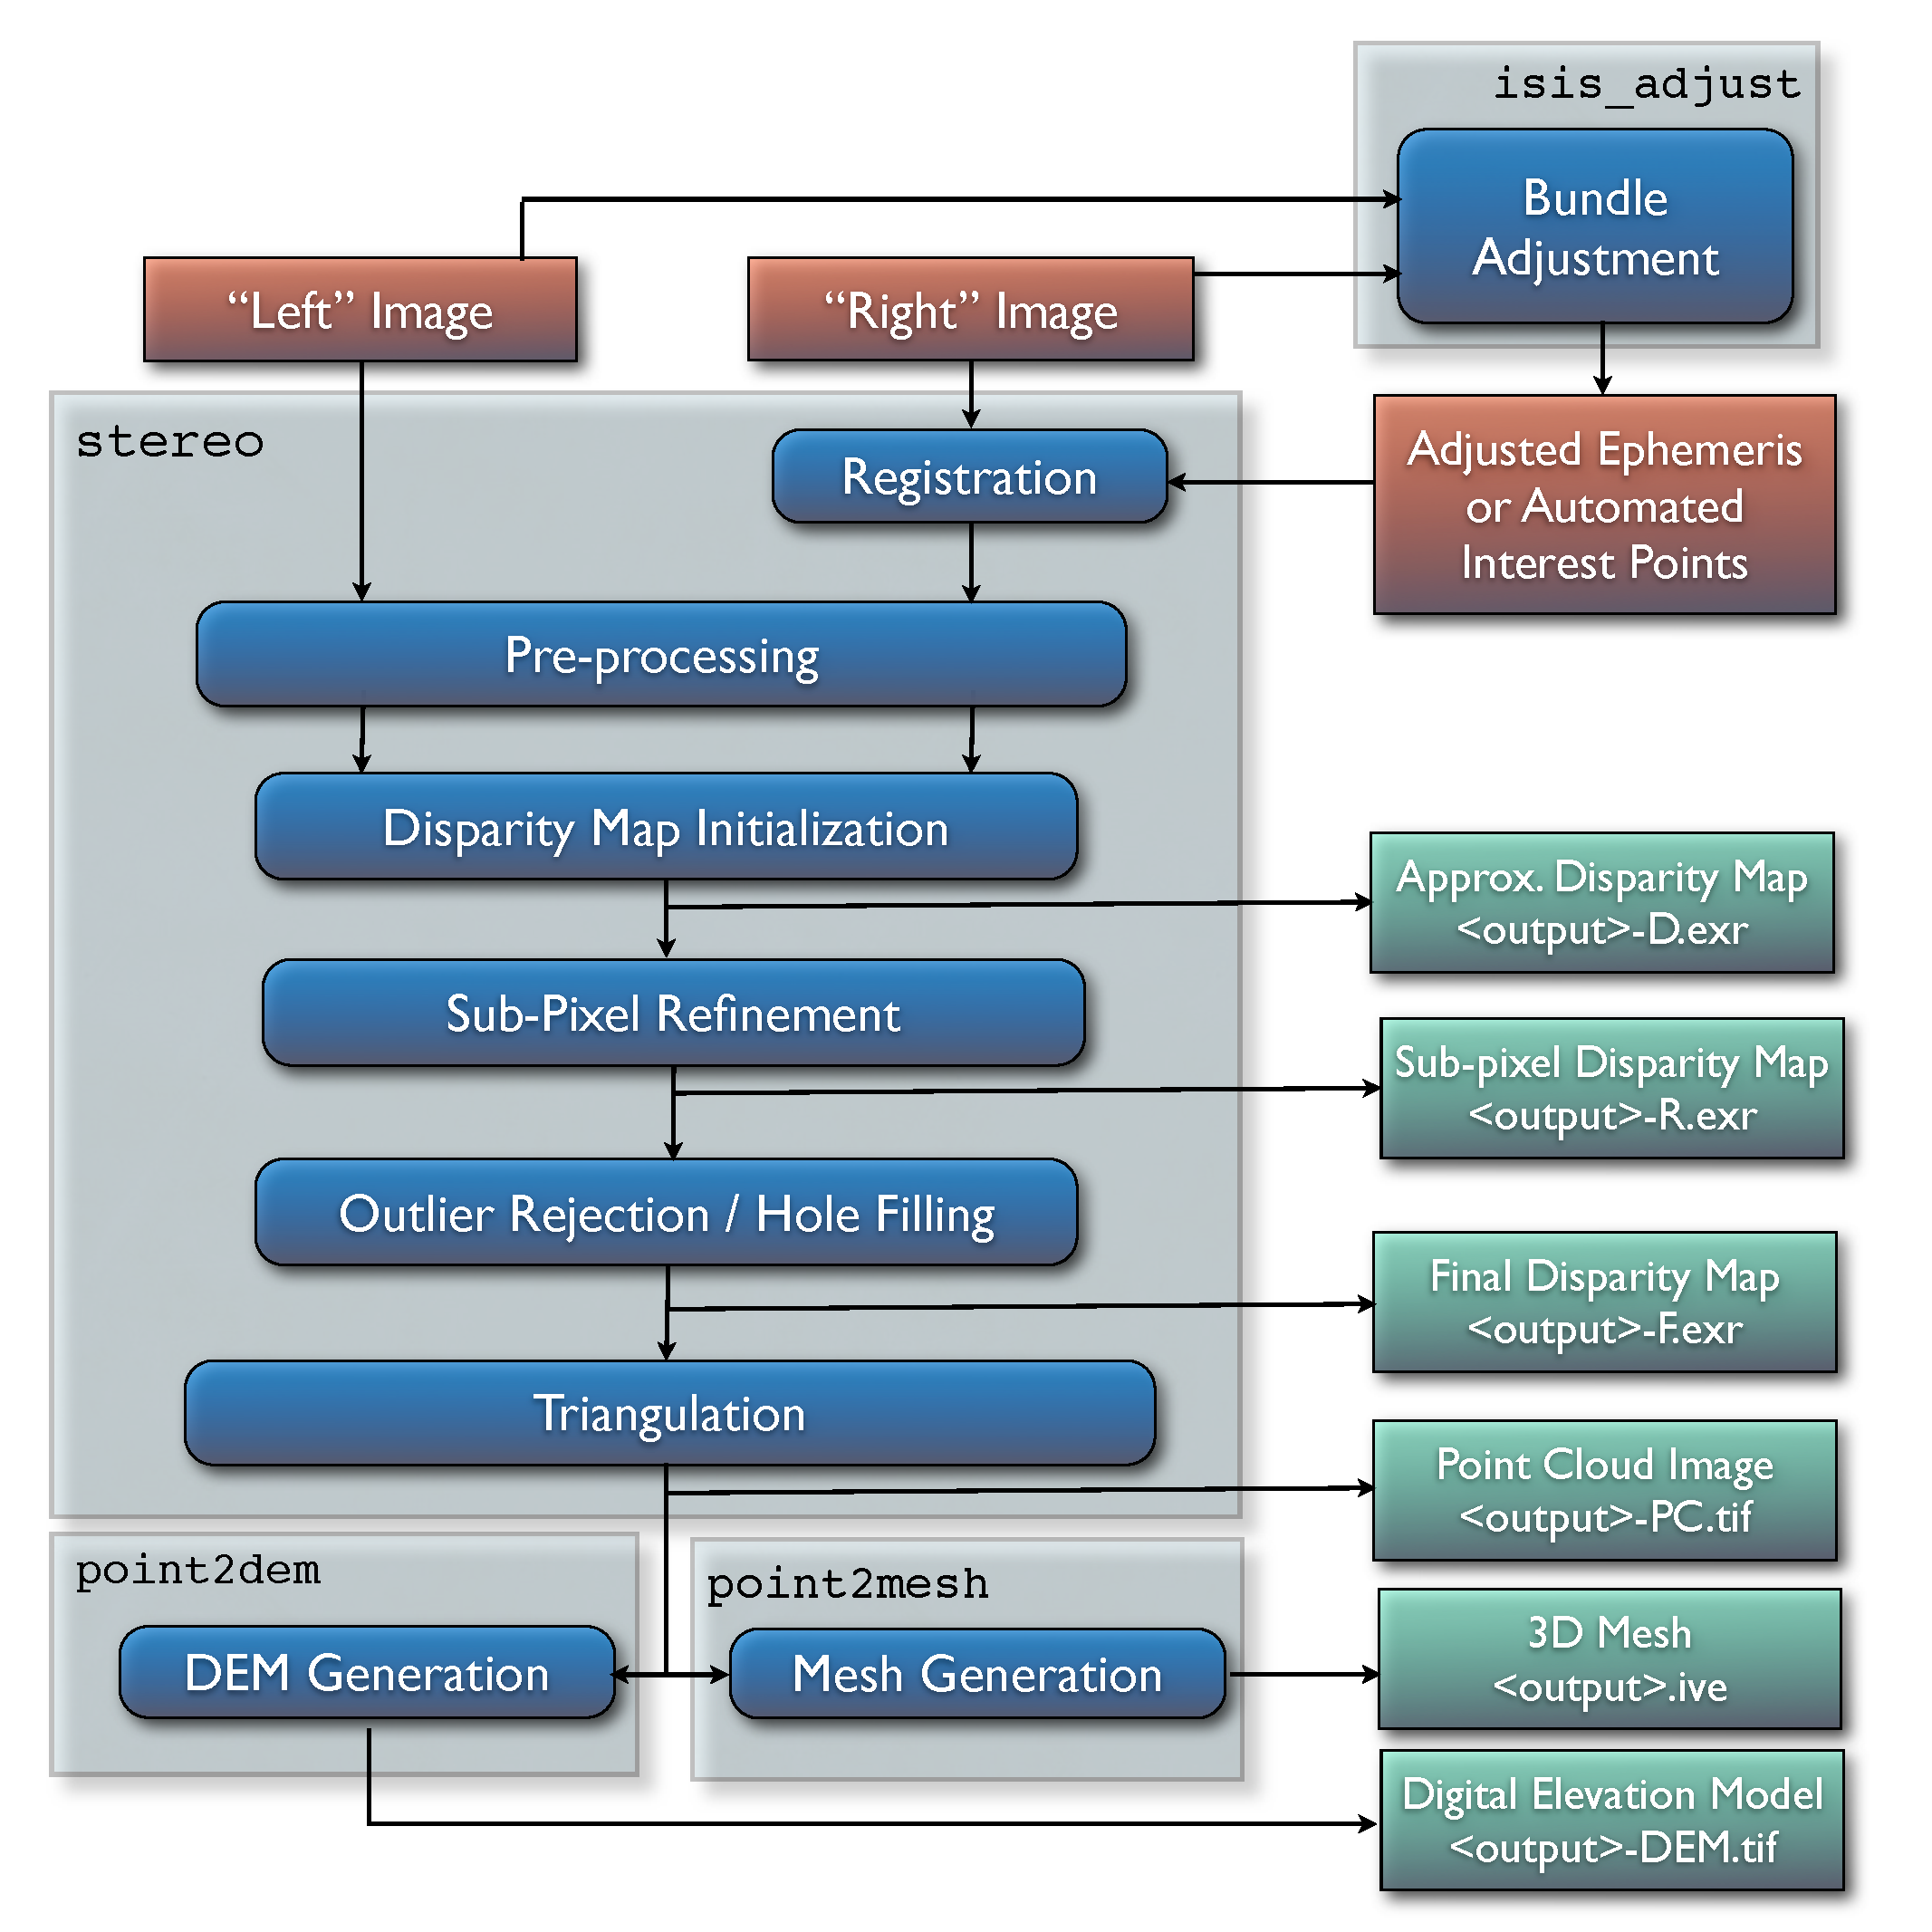
\includegraphics[width=7cm]{images/asp}
  \caption{Flow of data through the Ames Stereo Pipeline}
  \label{fig:asp}
\end{figure}

The process begins with least squares Bundle Adjustment, which is
described in Section~\ref{sec:bundle_adjustment}, below.  This
produces corrected extrinsic camera parameters that are utilized by
various camera modeling steps.

Then, the left and right images are aligned using interest points or
geometric constraints from the camera models.  This step is often
essential for performance because it ensures that the disparity search
space is bounded to a known area.  Next, a prepossessing filter such
as the Sign of the Laplacian of the Gaussian filter is used, which has
the effect of producing images that are somewhat invariant to
differences in lighting conditions~\cite{Nishihara84practical}.

Following these pre-processing steps, we compute the disparity space
image $DSI(i,j,d_x, d_y)$ that stores the matching cost between a left
image block centered around pixel $(i,j)$ and a right image block
centered at position $(i-d_x, j-d_y)$.  At this stage, the quality of
the match is measured as the normalized cross
correlation~\cite{Menard97:robust} between two 15x15 pixel image
patches.  We employ several optimizations to accelerate this
computation: (1) a box filter-like accumulator that reduces duplicate
operations in the calculation of $DSI$~\cite{Sun02rectangular}; (2) a
coarse-to-fine pyramid based approach where disparities are estimated
using low resolution images, and then successively refined at higher
resolutions; and (3) partitioning of the disparity search space into
rectangular sub-regions with similar values of disparity determined in
the previous lower resolution level of the
pyramid~\cite{Sun02rectangular}.

The $DSI$ estimate just described efficiently computes {\em integer}
estimates of disparity between the two images.  These estimates are
subsequently refined to sub-pixel accuracy using the technique
described in Section~\ref{sec:subpixel}.  Finally, in conjunction with
the bundle adjusted camera models, the sub-pixel disparity estimates
are used to triangulate the location of 3D points as the closest point
of intersection of two forward-projected rays emanating from the
centers of the two cameras through the matched pixels.


\section{Sub-pixel Stereo Correlation}\label{sec:subpixel}

Apollo images are affected by two types of noise inherent to the
scanning process: (1) the presence of film grain and (2) dust \& lint
particles.  The former gives rise to noise in the DEM values that wash
out real features, and the latter causes incorrect matches or hard to
detect blemishes in the DEM.  Attenuating the effect of these scanning
artifacts while simultaneously refining the integer disparity map to
sub-pixel accuracy has become a critical goal of our system, and is
necessary for processing real-world data sets such as the Apollo
Metric Camera data.

A common technique in sub-pixel refinement is to fit a parabola to the
correlation cost surface in the 8-connected neighborhood around the
integer disparity estimate, and then use the parabola's minimum as the
sub-pixel disparity value. This method is easy to implement and fast
to compute, but exhibits a problem known as pixel-locking: the
sub-pixel disparities tend toward their integer estimates and can
create noticable "stair steps" on surfaces that should be
smooth~\cite{Stein06:attenuating},~\cite{Szeliski03sampling}.  One way
of attenuating the pixel-locking effect is through the use of a
symmetric cost function~\cite{Nehab05:improved} for matching the
``left'' and ``right'' image blocks.  

To avoid the high computational complexity of these methods another
class of approaches based on the Lucas-Kanade
algorithm~\cite{Baker04:lucas-kanade} proposes an asymmetric score
where the disparity map is computed using the best matching score
between the left image block and an optimally affine transformed block
from the right image.  For example, the sub-pixel refinement developed
by Stein et. al.~\cite{Stein06:attenuating} lets $I_R(m,n)$ and
$I_L(i,j)$ be two corresponding pixels in the right and left image
respectively, where $i = m+d_x$, $j = n+d_y$ and $d_x, d_y$ are the
integer disparities.  They develop a linear approximation based on the
Taylor Series expansion around pixel $(i,j)$ in the left image
\begin{eqnarray}
I_L(i+\delta_x,j + \delta_y)\approx I_L(i,j) + \delta_x\frac{dI_L}{d_x}(i,j)+\delta_y\frac{dI_L}{d_y}(i,j) 
\label{taylor_expansion}
\end {eqnarray}
where $\delta_x$ and $\delta_y$ are the local sub-pixel displacements.
Let $e(x,y) = I_R(x,y) - I_L(i+\delta_x,j+\delta_y)$ and $W$ be an
image window centered around pixel $(m,n)$.  The local displacements
are not constant accross $W$ and they vary according to:
\begin{eqnarray}
\nonumber
\delta_x(i,j) = a_1i+b_1j+c_1\\
\delta_y(i,j) = a_2i+b_2j+c_2. 
\label{affine_transform}
\end {eqnarray}
The goal is to find the parameters $a_1, b_1, c_1, a_2, b_2, c_2$ that
minimize the cost function
\begin{eqnarray}
{\bf E}(m,n) =\sum_{(x,y)\in W} (e(x,y)w(x,y))^2
\label{affine2D_cost}
\end{eqnarray}
where $w(x,y)$ are a set of weights used to reject outliers. Note that
the local displacements $\delta_x(i,j)$ and $\delta_y(i,j)$ depend on
the pixel positions within the window $W$. In fact, the values $a_1,
b_1, c_1, a_2, b_2, c_2$ that minimize $\bf E$ can be seen as the
parameters of an affine transformation that best transforms the right
image window to match the reference (left) image window.

%In the original Lucas-Kanade method the weights are set
%$w(x,y)=1$. In~\cite{Stein06:attenuating} the values the weights
%$w(x,y)$ determined heuristically to reject the noise and emphasize
%the pixel closer to the center of the window. An alternative solution
%is to use a set of constant weights derived from the Cauchy
%distribution~\cite{Menard97:robust} given by: \begin{eqnarray}
%w(x,y)= \frac{\sqrt{b^2 \log(1+\frac{I_e^2(x,y)}{b^2})}
%}{|I_e(x,y)|} \label{Cauchy_weights} \end{eqnarray} where $b$ is some
%fixed threshold (in our experiments $b = 10^{-4}$) and $I_e(x,y) =
%I_R(x,y)-I_L(i,j)$.
 
%The steps of this method are given below
%\begin{itemize}
%\item {\bf Step 1:} Compute $\frac{dI_L}{d_x}(i,j)$, $\frac{dI_L}{d_y}(i,j)$ and the $I_R(x,y)$ values using bilinear interpolation. Initialize the parameters $a_1, b_1, c_1, a_2, b_2, c_2$.
%\item {\bf Step 2:} Determine ${a_1, b_1, c_1, a_2, b_2, c_2}$ to minimize ${\bf E}$. 
%\item {\bf Step 3:} Compute $\delta_x(i,j)$ and $\delta_y(i,j)$ using Equation~\ref{affine_transform}.
%\item {\bf Step 4:} Compute a new point $(x', y') = (x, y) + (\delta_x, \delta_y)$ and the $I_R(x',y')$ values using bilinear interpolation.
%\item {\bf Step 5:} Check for convergence. If norm of ($\delta_x, \delta_y$) vector falls below a fixed threshold the iterations converged. Otherwise, go to step 1.
%\end{itemize}

The shortcoming of this method is directly related to the cost
function that it is minimizing, which has a low tolerance to noise.
Noise present in the image will easily dominate the result of the
squared error function, giving rise to erroneous disparity
information.  Recently, several statistical
approaches (e.g. ~\cite{cheng04:bayesian}) have emerged to show how
stochastic models can be used to attenuate the effects of noise.  Our
sub-pixel refinement technique~\cite{Nefian09:bayesian} adopts some of
these ideas, generalizing the earlier work by Stein
et. al.~\cite{Stein06:attenuating} to a Bayesian framework that models
both the data and image noise.

%\begin{eqnarray}
%\nonumber
%{\bf E}(m,n))&=& \sum_{(x,y)\in W}((I_R(x,y) - I_L(i+\delta_x, j+\delta_y))^2\\
%\nonumber
%\tilde{\delta_x} &=& \arg \min_{\delta_x} {\bf E}(m,n)\\
%\nonumber
%\tilde{\delta_y} &=& \arg \min_{\delta_x} {\bf E}(m,n)\\
%\nonumber           
%P({\bf I}_R(m,n))&=&\prod_{(x,y)\in W}{\cal N}(I_R(x,y)|I_L(i+\delta_x, j+\delta_y), \sigma_p)P(k=0)\\
%\nonumber
%                 &+&{\cal N}(I_R(x,y)|\mu_n, \sigma_n)P(k=1)\\
%\nonumber
%\tilde{\delta_x} &=& \arg \max_{\delta_x} P({\bf I}_R(m,n))\\
%\nonumber
%\tilde{\delta_y} &=& \arg \max_{\delta_y} P({\bf I}_R(m,n))\\
%\nonumber
%m &=& m+\tilde{\delta_x}\\
%\nonumber
%n &=& n+\tilde{\delta_y}
%\end{eqnarray}

In our approach the probability of a pixel in the right image is given
by the following Bayesian model:
\begin{eqnarray}
P(I_R(m,n))&=& \prod_{(x,y)\in W}{\cal N}(I_R(m,n)|I_L(i+\delta_x, j+\delta_y), \frac{\sigma_p}{\sqrt{g_{xy}}})P(z=0) + \\
\nonumber
           &+& {\cal N}(I_R(m,n)|\mu_n, \sigma_n)P(z=1)
\label{pix}
\end {eqnarray}
The first mixture component $(z=0)$ is a normal density function with
mean $I_L(i+\delta_x, j+\delta_y)$ and variance $\frac{\sigma_p}{\sqrt{g_{xy}}}$:
\begin{eqnarray}
P(I_R(m,n)|z=0) = {\cal N}(I_R(m,n)|I_L(i+\delta_x, j+\delta_y), \frac{\sigma_p}{\sqrt{g_{xy}}})
\label{pixel_stereo_model}
\end {eqnarray}
The $\frac{1}{\sqrt{g_{xy}}}$ factor in the variance of this component
has the effect of a Gaussian smoothing window over the patch. With
this term in place, we are no longer looking for a single variance
over the whole patch; instead we are assuming the variance increases
with distance away from the center according to the inverted Gaussian,
and are attempting to fit a global scale, $\sigma_p$. This provides
formal justification for the standard Gaussian windowing kernel.

The second mixture component $(z=1)$ in
Equation~\ref{pixel_stereo_model} models the image noise using a
normal density function with mean $\mu_n$ and variance $\sigma_n$:
\begin{eqnarray}
P(I_R(m,n)|z=1) = {\cal N}(I_R(m,n)|\mu_n, \sigma_n)
\label{pixel_noise_model}
\end {eqnarray}
Let ${\bf I}_R(m,n)$ be a vector of all pixels values in a window $W$
centered in pixel $(m,n)$ in the right image. Then,
\begin{eqnarray}
P({\bf I}_R(m,n)) = \prod_{(x,y)\in W}P(I_R(x,y))
\label{bayes_model}
\end {eqnarray}

The parameters $\lambda = \{a_1, b_1, c_1, a_2, b_2, c_2,
\sigma_p,\mu_n, \sigma_n\}$ that maximize the model likelihood in
Equation~\ref{bayes_model} are determined using the Expectation
Maximization (EM) algorithm. Maximizing the model likelihood in
Equation~\ref{bayes_model} is equivalent to maximizing the auxiliary
function:
\begin{eqnarray}
\nonumber
{\bf Q(\theta)}&=& \sum_k P(k|{\bf I}_R, \lambda_t) \log P ({\bf I}_R, k, {\underline \delta}|\lambda)\\
&=& \sum_{k}\sum_{x,y} P(k|I_R(x,y), \lambda_t)\log P (I_R(x,y)|k, \lambda)P(k|\lambda)
\label{aux_function}
\end {eqnarray}

Note that the M step calculations are similar to the equation used to
determine the parameters $a_1, b_1, c_1, a_2, b_2, c_2$ in the method
presented in~\cite{Stein06:attenuating}, except here the fixed set of
weights is replaced by the a posteriori probabilities computed in the
E step. In this way, our approach can be seen as a generalization of
the Lucas-Kanade method.  The complete algorithm is summarized in the following steps:
\begin{itemize}
\item {\bf Step 1:} Compute $\frac{dI_L}{d_x}(i,j)$, $\frac{dI_L}{d_y}(i,j)$ and the $I_R(x,y)$ values using bilinear interpolation. Initialize the model parameters $\lambda$.
\item {\bf Step 2:} Compute iteratively the model parameters $\lambda$ using the EM algorithm (see ~\cite{Nefian09:bayesian} for details). 
\item {\bf Step 3:} Compute $\delta_x(i,j)$ and $\delta_y(i,j)$ using Equation~\ref{affine_transform}.
\item {\bf Step 4:} Compute a new point $(x', y') = (x, y) + (\delta_x, \delta_y)$ and the $I_R(x',y')$ values using bilinear interpolation.
\item {\bf Step 5:} If the norm of ($\delta_x, \delta_y$) vector falls below a fixed threshold the iterations converged. Otherwise, go to step 1.
\end{itemize}

\begin{figure}[bt]
  \begin{center}
%    \subfigure[]{\includegraphics[width=6cm]{images/orbit33}}
%    \subfigure[]{\includegraphics[width=6cm]{images/apollo_3D}}
    \caption{Hadley Rille and the Apollo 15 landing site derived from
      Apollo Metric Camera frames AS15-M-1135 and AS15-M-1136. (a)
      superimposed over the USGS Clementine base map, (b) oblique view.}
    \label{results_crater_img}
  \end{center}
\end{figure} 

Like the computation of the integer $DSI$, we adopt a multi-scale
approach for sub-pixel refinement. At each level of the pyramid, the
algorithm is initialized with the disparity determined in the previous
lower resolution level of the pyramid. This allows the subpixel
algorithm to shift the results of the integer $DSI$ by many pixel if
a better match can be found using the affine, noise-adapted window.


%-----

This chapter provides a graphical representation of how correlation is
performed in Ames Stereo Pipeline. Most importantly this provides a
quick comparison of different algorithms provided to save the user the
time of comparing results themselves.

For this chapter we'll be using the north most tip of Hadley Rille as
captured by the Apollo 15 Metric Camera. Here's what the left and right
pair looks like before any processing has been applied. The right image
is actually larger than the left.

\begin{figure}[hb]
\centering
  \subfigure[{\tt Left}]{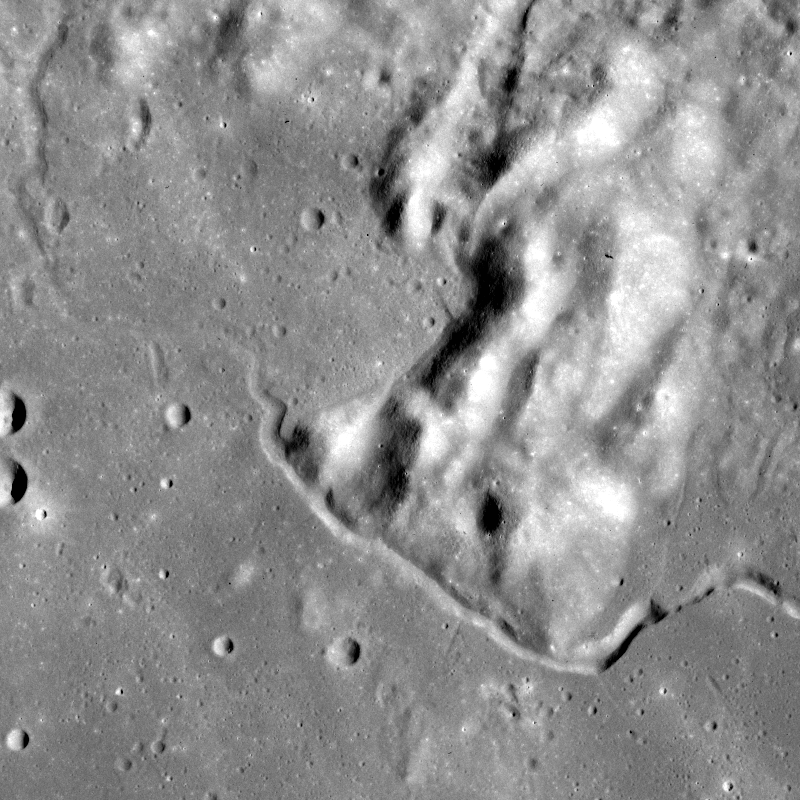
\includegraphics[width=3in]{images/correlation/sub4-AS15-M-1134_crop.png}\label{fig:left_input_image}}
  \hfil
  \subfigure[{\tt Right}]{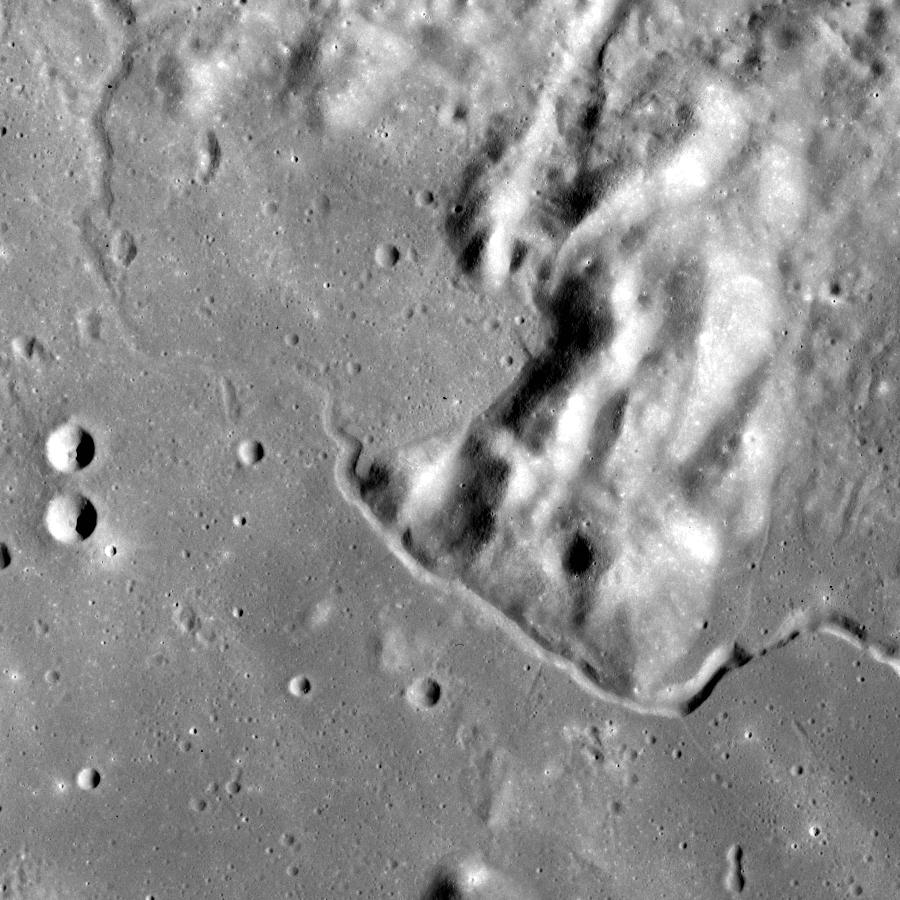
\includegraphics[width=3in]{images/correlation/sub4-AS15-M-1135_crop.png}\label{fig:right_input_image}}
\caption{Original input images used for this chapter.}
\label{fig:input_images}
\end{figure}

\section{Preprocessing Filters and Integer Correlation}
\label{sec:prefilter_n_correlation}

\subsection{Cost Functions}

\subsection{Gaussian Blur}

\subsection{Log Filter}

\subsection{SLog Filter}

\subsection{Pyramid Correlator}

\section{Sub-pixel Correlation}
\label{sec:subpixel_correlation}

\subsection{Parabola}

\begin{figure}[hb]
\centering
  \subfigure[{\tt 3D result}]{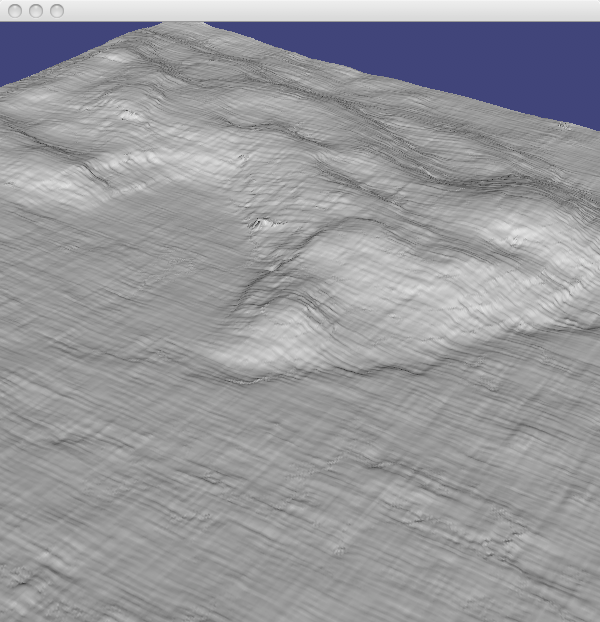
\includegraphics[width=3in]{images/correlation/3D_mode0.png}}
  \hfil
  \subfigure[{\tt Hillshade Result}]{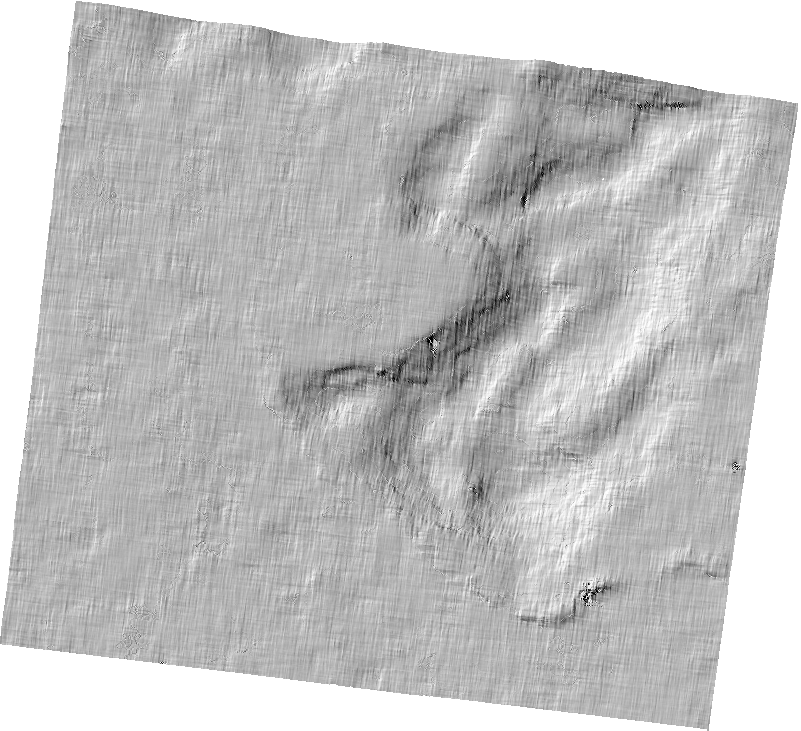
\includegraphics[width=3in]{images/correlation/hillshade_mode0.png}}
\caption{Results using Parabola subpixel mode.}
\label{fig:parabola_results}
\end{figure}

\subsection{Robust weighted Affine}

\begin{figure}[hb]
\centering
  \subfigure[{\tt 3D result}]{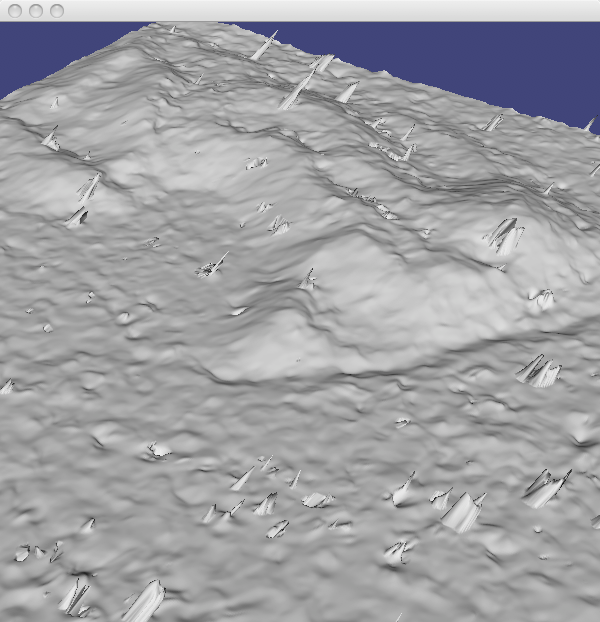
\includegraphics[width=3in]{images/correlation/3D_mode1.png}}
  \hfil
  \subfigure[{\tt Hillshade Result}]{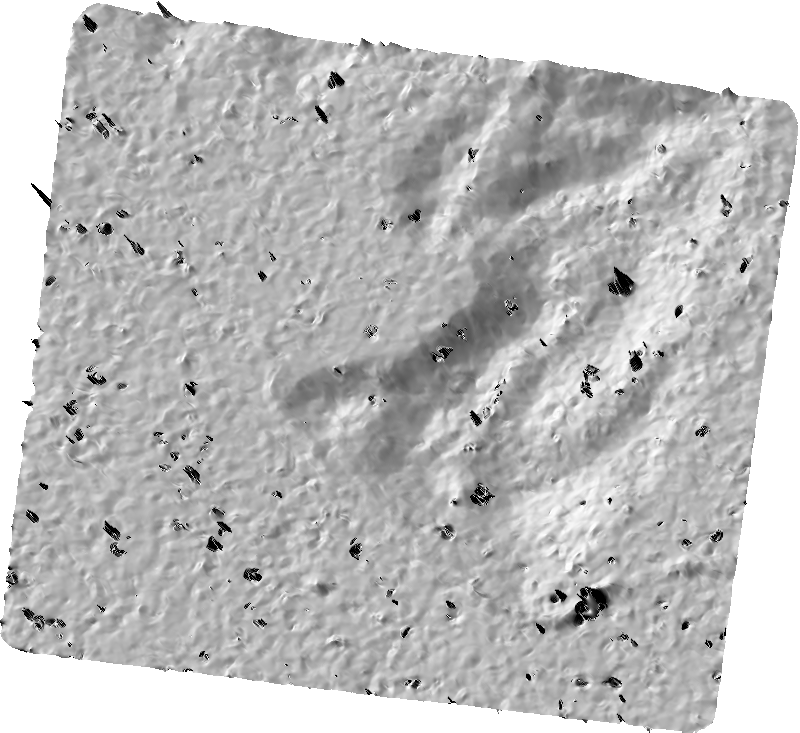
\includegraphics[width=3in]{images/correlation/hillshade_mode1.png}}
\caption{Results using Robust Affine subpixel mode.}
\label{fig:robust_results}
\end{figure}

\subsection{Bayes weighted Affine}

\begin{figure}[hb]
\centering
  \subfigure[{\tt 3D result}]{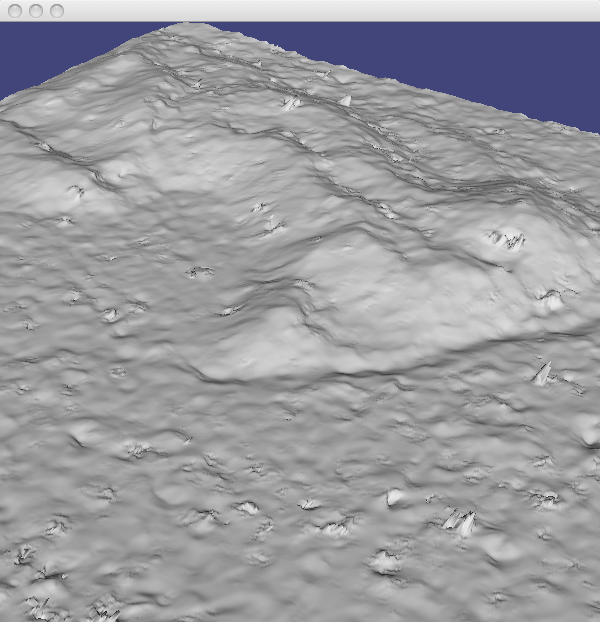
\includegraphics[width=3in]{images/correlation/3D_mode2.png}}
  \hfil
  \subfigure[{\tt Hillshade Result}]{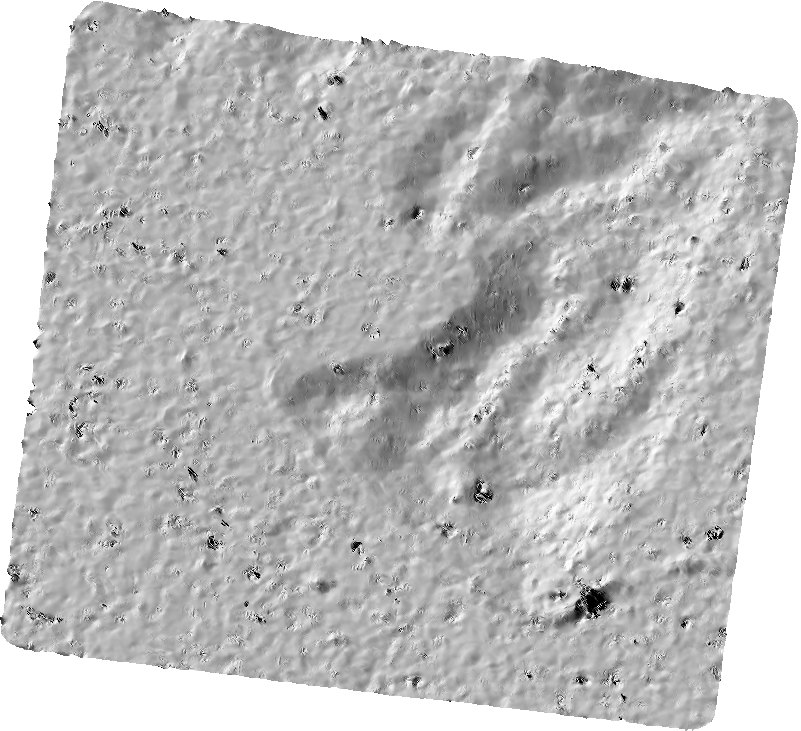
\includegraphics[width=3in]{images/correlation/hillshade_mode2.png}}
\caption{Results using Bayes weighted Affine subpixel mode.}
\label{fig:bayes_results}
\end{figure}

\subsection{Bayes EM weighted Affine}

\begin{figure}[hb]
\centering
  \subfigure[{\tt 3D result}]{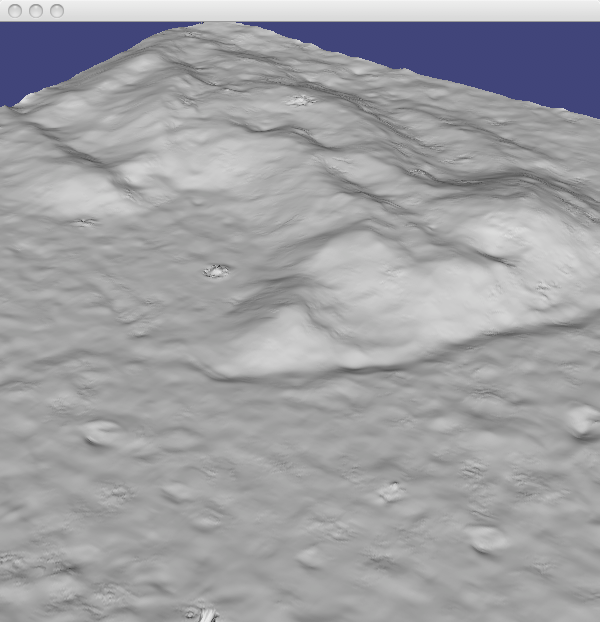
\includegraphics[width=3in]{images/correlation/3D_mode3.png}}
  \hfil
  \subfigure[{\tt Hillshade Result}]{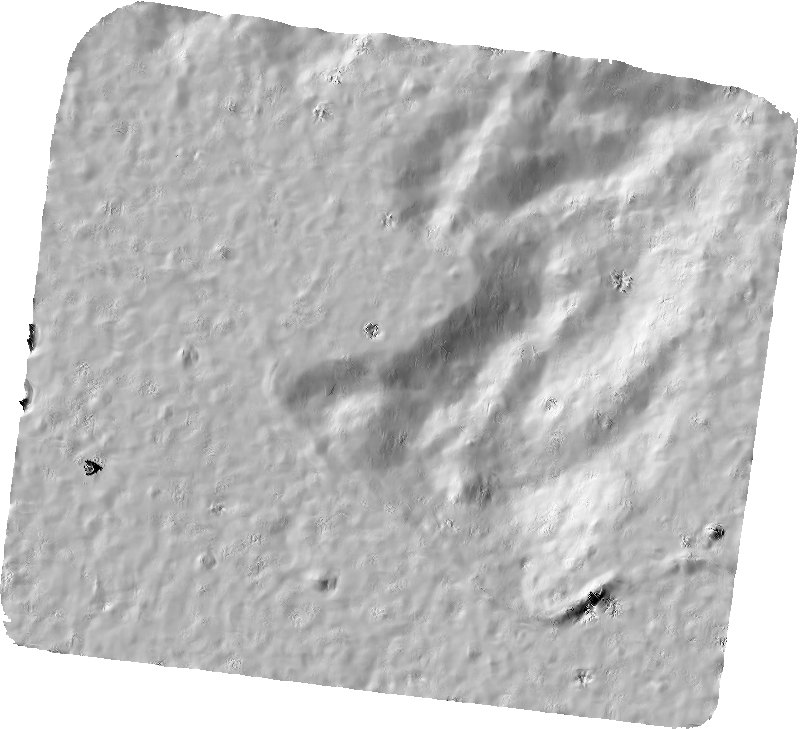
\includegraphics[width=3in]{images/correlation/hillshade_mode3.png}}
\caption{Results using Bayes EM weighted Affine subpixel mode.}
\label{fig:bayes_em_results}
\end{figure}
